\section{Detection of objects in LiDAR: challenges}%New title
Traditional work in object detection focusses on what we will call "natural images", which are photographs of scenes seen in normal settings. For examples, people sitting at a table, or children in front of horses. They are similar to images we would see with our own eyes. This means that, if there is an object in a photograph, there is a high probability that this object also exist and is the same category in the real scene that has been photographed. In other words, there is a good correspondence between the real object, its classification, and the kind of signal it emits in the visual field. A photograph of a camel will contain a camel, and we are able to very confidently classify the image as containing a camel, even though we are only classifying a \textit{visual representation}, not the object itself.

\begin{figure}[h]
	\begin{subfigure}[t]{.5\textwidth}
  \centering
  % include first image
  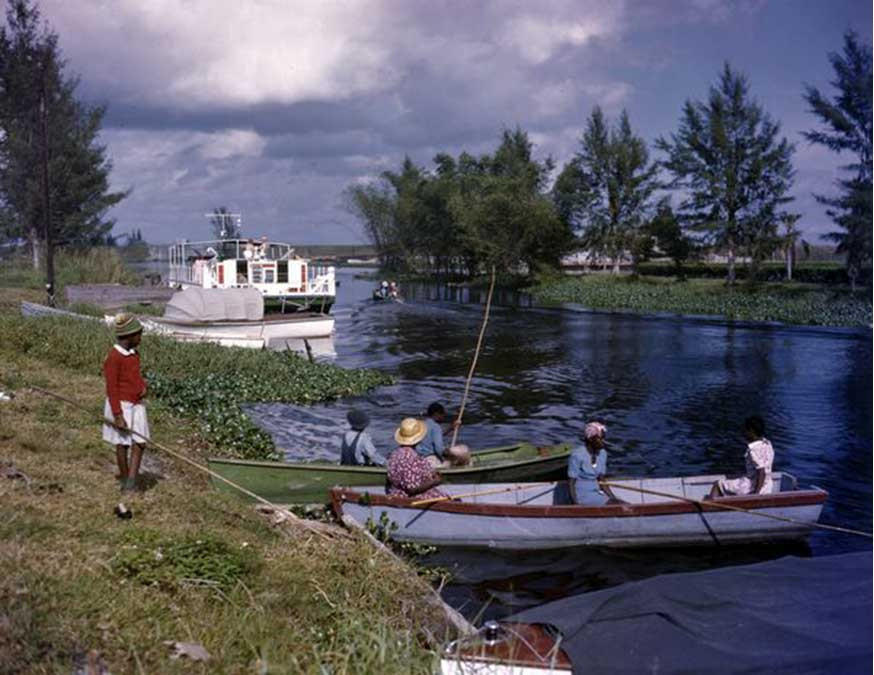
\includegraphics[width=\linewidth]{coco}  
	\caption{A natural image, taken from the COCO\cite{msCOCO} dataset}
  \label{fig:cocoEx}
\end{subfigure}
	\begin{subfigure}[t]{.5\textwidth}
  \centering
  % include second image
  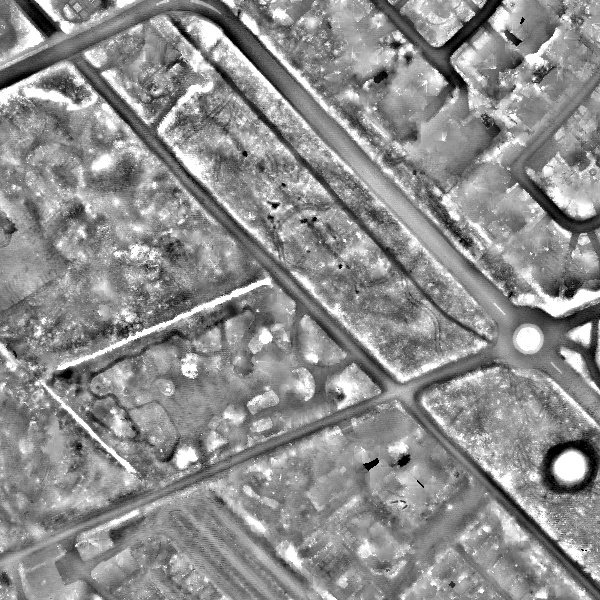
\includegraphics[width=\linewidth]{lidarEx}  
  \caption{An example from the LiDAR dataset. On the bottom right, we can see an example of a barrow. However, this barrow is very similar to the roundabount seen slightly above.}
  \label{fig:lidarEx}
\end{subfigure}
	\caption{A natural image \textit{versus} a LiDAR survey}
\label{fig:cocovslidar}
\end{figure}

In geophysical surveys, or more generally with any kind of image that is not made of purely visible light, the difference between the representation and the real object is more pronounced, and while it might be easy to detect and classify objects in the representation, to guarantee that those detected objects always match up with a real object is much more tricky. How can we say that the white mass seen in an X-Ray scanner that we detect and classify as a tumor is not only indeed a tumor in its representation, but also match up with a real tumor in a patient? The problem is even more prevalent with geophysical data, with noise and geological details adding yet another layer of complexity.

Other issues that are specific and prevalent in geophysical data are the size and resolution of the images. Whereas in natural images might be around a thousand pixels in width, geophysical surveys cover hundreds of kilometer square of area, and are often tens of thousands of pixels wide. Moreover, the size of the object to detect is tiny in comparison to the size of the image, which is not usually the case in natural images. Traditional object detection techniques take advantage of this by heavily downscaling the image through the layers of the network, greatly reducing the computational cost. This is not possible to do with geophysical surveys: a barrow, which might be a few meters wide in reality will be only a few pixels wide, and by downscaling we might lose all informations concerning those small objects. 

When working with geophysical data, one must always keep in mind those issues. In our case, the only reliable way of classifying archaelogical objects is by prospection and physical inspection, something that \textbf{cannot be done using only geophysical surveys}. However, this create another issue, one of scale. In the dataset that I had at my disposition, more than hundreds of kilometers squared were surveyed and contains more than 3000 objects of different classes. It is almost impossible to verify for every object if they are of the correct classification by way of prospecting: it is too costly and too much time consuming. 

In short, even if the annotations in the dataset are entirely correct, something that is very hard to confirm, and even if the network architecture is fit for the task and trained well, something that is even harder to do, we will still have an incertainty as to wether the detected object are not only actually real, but of the correct class. 

\section{Dataset}\label{diffDataset}
In of itself, it is quite challenging to obtain large segments of LiDAR surveys, or for that matter any kind of geophysical surveys. Deep Learning techniques usually requires vast amount of data to train properly. However, here  data can be prohibitively expensive to produce: a geophysical survey of an area is itself a challenge, with funding to secure and plannification to be done. 

In Archaelogy, the practice of Open Data, the act of freely sharing the data produced, is not yet widely adopted for a multitude of reasons. 

